% gm-02-LinearEqs.tex

\documentclass[xcolor=dvipsnames]{beamer}

\usepackage{cancel}
\renewcommand{\CancelColor}{\color{red}}
\usepackage{graphicx}
\usepackage{wrapfig}
\usepackage{colortbl}
\usepackage{color}
\usepackage{alltt}
\renewcommand*{\thefootnote}{\fnsymbol{footnote}}
\definecolor{myblue}{rgb}{0.8,0.85,1}

\mode<presentation>
{
  \usetheme{Warsaw}
  \setbeamercovered{transparent}
}
% \usecolortheme[named=OliveGreen]{structure}
\setbeamertemplate{navigation symbols}{} 
\setbeamertemplate{blocks}[rounded][shadow=true] 

% this is for overlaying math symbols, see https://tex.stackexchange.com/questions/12895/overlay-symbol-with-another
\def\qeq{\mathrel{%
    \mathchoice{\QEQ}{\QEQ}{\scriptsize\QEQ}{\tiny\QEQ}%
}}
\def\QEQ{{%
    \setbox0\hbox{$\longrightarrow$}%
    \rlap{\hbox to \wd0{\hss/\hss}}\box0
  }}

\newcounter{expls}
\setcounter{expls}{0}
\newcommand{\beispiel}[1]{\refstepcounter{expls}\textbf{Example \arabic{expls}: #1.}}

\newcounter{exercise}
\setcounter{exercise}{0}
\newcommand{\ubung}[0]{\refstepcounter{exercise}\textbf{Exercise \arabic{exercise}: }}

\newif\ifBCITCourse
\BCITCoursetrue
% \BCITCoursefalse
\newif\ifWhichCourse
\WhichCoursetrue
\WhichCoursefalse
\ifBCITCourse
\ifWhichCourse
\newcommand{\CourseName}{Technical Mathematics for Food Technology}
\newcommand{\CourseNumber}{MATH 1441}
\newcommand{\CourseInst}{BCIT}
\else
\newcommand{\CourseName}{Technical Mathematics for Geomatics}
\newcommand{\CourseNumber}{MATH 1511}
\newcommand{\CourseInst}{BCIT}
\fi
\else
\newcommand{\CourseName}{Philosophy and Literature}
\newcommand{\CourseNumber}{PHIL 375}
\newcommand{\CourseInst}{UBC}
\fi

\title{Scientific Notation and Linear Equations}
\subtitle{{\CourseNumber}, BCIT}

\author{\CourseName}

\date{September 7, 2017}

\begin{document}

\begin{frame}
  \titlepage
\end{frame}

\begin{frame}
  \frametitle{Significant Digits}
  Determine the number of significant digits in the following
  measurements:

\bigskip

  \begin{tabular}{rcl}
    587$m$ & \hspace{.5in} & \textcolor{white}{3 significant digits} \\
    890.8$m$ & \hspace{.5in} & \textcolor{white}{4 significant digits} \\
    30.7$^{\circ}$ & \hspace{.5in} & \textcolor{white}{3 significant digits} \\
    800$km$ & \hspace{.5in} & \textcolor{white}{1 significant digit} \\
    0.080$N$ & \hspace{.5in} & \textcolor{white}{2 significant digits} \\
    0.0801$N$ & \hspace{.5in} & \textcolor{white}{3 significant digits} \\
    0.0800$N$ & \hspace{.5in} & \textcolor{white}{3 significant digits} \\
  \end{tabular}
\end{frame}

\begin{frame}
  \frametitle{Significant Digits}
  Determine the number of significant digits in the following
  measurements:

\bigskip

  \begin{tabular}{rcl}
587$m$ & \hspace{.5in} & 3 significant digits \\
890.8$m$ & \hspace{.5in} & 4 significant digits \\
30.7$^{\circ}$ & \hspace{.5in} & 3 significant digits \\
800$km$ & \hspace{.5in} & 1 significant digit\footnote{Perhaps we are unlucky and there are actually 2 or 3 significant digits. One significant digit is the best guess based on the information that we have.} \\
0.080$N$ & \hspace{.5in} & 2 significant digits\footnote{Again there is an ambiguity here: it may be 3 significant digits.} \\
0.0801$N$ & \hspace{.5in} & 3 significant digits \\
0.0800$N$ & \hspace{.5in} & 3 significant digits\footnote{Note here that it is important to add the zeroes in order to indicate the number of significant digits. There is a subtle difference between $0.8$ and $0.800$.} \\
  \end{tabular}
\end{frame}

\begin{frame}
  \frametitle{Scientific Notation}
  In order to deal with significant digits in a consistent manner,
  we use scientific notation. A number in scientific notation will
  always be of the form
  \begin{equation}
    \label{eq:saegahni}
    p\times{}10^{n}
  \end{equation}
where $n\in\mathbb{Z}$ and $p\in\{x\in\mathbb{R}|1\leq{}x<10\}$.

\bigskip

We use the \textsc{EEX} button on our calculator to input numbers in
scientific notation.
\end{frame}

\begin{frame}
  \frametitle{Scientific Notation}
{\ubung} Express the following numbers in scientific notation; indicate the number of significant figures of each measurement.
\begin{itemize}
\item The radius of the earth is 6378.1$km$
\item The speed of light is $299792458m/s$
\item The radius of Mars is 3397000$m$
\item The radius of a red blood cell is 0.00034$mm$
\end{itemize}
\end{frame}

\begin{frame}
  \frametitle{Scientific Notation}
    \begin{figure}[h]
    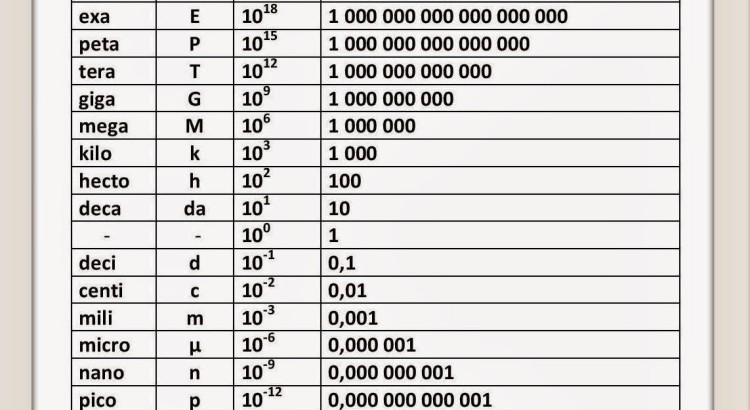
\includegraphics[scale=0.5]{./tabel.jpg}
  \end{figure}
\end{frame}

\begin{frame}
  \frametitle{Scientific Notation}
{\ubung} Solve the following problems.
\begin{itemize}
\item At sea level, atmospheric pressure is about 101300$Pa$.  How
  many $kPa$ is this?
\item A weather satellite orbiting the Earth has a mass of
  2200$kg$. How many grams is this?
\item A microbe has a diameter of 3$\mu{}m$. How many $mm$ is
  this?
\item The mass of the moon is $7.346\times{}10^{22}kg$. Express
  this value in grams.
\item The mass of an electron is $9.109\times{}10^{-31}kg$.
  Express this value in grams.
\end{itemize}
\end{frame}

\begin{frame}
  \frametitle{Scientific Notation}
{\ubung} Solve the following problems.
\begin{itemize}
\item The Moon travels about $2400000km$ in about 28 days in one rotation
  about the Earth. Express the Moon's velocity in $m/s$.
\item A commercial jet with 230 passengers on a $2850km$ flight from Vancouver to
  Chicago averaged $765km/h$ and used fuel at a rate of $5650L/h$.
  \begin{itemize}
  \item How many hours was the flight?
  \item How long, in seconds did it take to use $1.0L$ of fuel?
  \item What was the fuel consumption in $km/L$?
  \item What was the fuel consumption in $L/$passenger?
  \end{itemize}
\end{itemize}
\end{frame}

\begin{frame}
  \frametitle{Equations}
  {\ubung} Determine the solution set.
\begin{equation}
  \label{eq:b2}
  \begin{array}{rcl}
    8+x&=&13 \\ 
    x^{2}&=&4 \\ 
    \frac{x}{1}&=&x \\ 
    x+2&=&x \\ 
    \frac{x-7}{x-7}&=&1 \\ 
    \sqrt{x+1}&=&x-5 \\ 
  \end{array}\notag
\end{equation}
\end{frame}

\begin{frame}
  \frametitle{Equations}
  \addtocounter{exercise}{-1}
  {\ubung} Determine the solution set.
\begin{equation}
  \label{eq:b2a}
  \begin{array}{rcll}
    8+x&=&13&\alert{S=\{5\}} \\ 
    x^{2}&=&4&\alert{S=\{-2,2\}} \\ 
    \frac{x}{1}&=&x&\alert{S=\mathbb{R}} \\ 
    x+2&=&x&\alert{S=\{\}} \\ 
    \frac{x-7}{x-7}&=&1&\alert{S=\mathbb{R}\setminus\{7\}} \\ 
    \sqrt{x+1}&=&x-5&\alert{S=\{8\},\mbox{ NOT }S=\{3,8\}} \\ 
  \end{array}\notag
\end{equation}
\end{frame}

\begin{frame}
  \frametitle{Linear Equations}
An equation is said to be linear if the variable appears at most to the
power of $1$. Here are some examples,
\begin{equation}
  \label{eq:oothahlo}
  \begin{array}{rcl}
8x-6&=&12 \\
\hspace{.5in} && \\
3(p-5)&=&8 \\
\hspace{.5in} && \\
4-3(t-5)&=&9t
  \end{array}
\end{equation}
\end{frame}

\begin{frame}
  \frametitle{Linear Equations}
An equation is said to be linear if the variable appears at most to the
power of $1$. Here are some examples,
\begin{equation}
  \label{eq:auxaiboz}
  \begin{array}{rcll}
8x-6&=&12&\alert{S=\left\{\frac{9}{4}\right\}} \\
\hspace{.5in} &&& \\
3(p-5)&=&8&\alert{S=\left\{\frac{23}{3}\right\}} \\
\hspace{.5in} &&& \\
4-3(t-5)&=&9t&\alert{S=\left\{\frac{19}{12}\right\}}
  \end{array}
\end{equation}
\end{frame}

\begin{frame}
  \frametitle{Doing the Same Thing to Both Sides I}
Here is a proof that $1=2$. Let $a$ and $b$ be some real numbers for
which we know that they are not zero and that they are equal, so
$a,b\neq{}0$ and $a=b$. Then
\begin{equation}
  \label{eq:fdlsjfjj}
  \begin{array}{rclcl}
    a&=&b&|&\cdot{}a \\
    a^{2}&=&ab&|&-b^{2} \\
    a^{2}-b^{2}&=&ab-b^{2}&|&\mbox{factor} \\
    (a+b)(a-b)&=&b(a-b)&|&\div{}(a-b) \\
    a+b&=&b&|&\mbox{replace }a\mbox{ by }b \\
    b+b&=&b&|&\mbox{simplify} \\
    % 2b&=&b&|&\div{}b\mbox{ note that }b\neq{}0 \\
    2b&=&b&|&\div{}b \\
    2&=&1&& \\
  \end{array}
\end{equation}
\end{frame}

\begin{frame}
  \frametitle{Doing the Same Thing to Both Sides II}
  The key to solving equations is to \alert{do the same thing to both
    sides}. Let $A,B,D$ be any mathematical expressions. Then
\begin{equation}
  \label{eq:iughaijo}
  A=B
\end{equation}
is equivalent to
\begin{equation}
  \label{eq:ieraechi}
  \begin{array}{rcl}
    A+D&=&B+D \\
    A-D&=&B-D \\
    A\cdot{}D&=&B\cdot{}D \\
    \frac{A}{D}&=&\frac{B}{D} \\
  \end{array}
\end{equation}
although for the latter two it is important that $D\neq{}0$,
otherwise the relevant function $F$ applied to both sides is not
bijective.
\end{frame}

\begin{frame}
  \frametitle{Doing the Same Thing to Both Sides III}
Are the following also equivalent to $A=B$?
\begin{equation}
  \label{eq:uozingei}
  \begin{array}{rcl}
    A^{2}&=&B^{2} \\
\hspace{.5in} && \\
    |A|&=&|B| \\
\hspace{.5in} && \\
    \sqrt{A}&=&\sqrt{B}
  \end{array}
\end{equation}
\end{frame}

\begin{frame}
  \frametitle{Doing the Same Thing to Both Sides III}
Are the following also equivalent to $A=B$?
\begin{equation}
  \label{eq:upohngee}
  \begin{array}{rcll}
    A^{2}&=&B^{2}&\alert{\mbox{no, use with caution}} \\
\hspace{.5in} &&& \\
    |A|&=&|B|&\alert{\mbox{no, use with caution}} \\
\hspace{.5in} &&& \\
    \sqrt{A}&=&\sqrt{B}&\alert{\mbox{no, use with caution}}
  \end{array}
\end{equation}
\end{frame}

\begin{frame}
  \frametitle{Doing the Same Thing to Both Sides IV}
Consider the following:
\begin{equation}
  \label{eq:oopiesho}
  \begin{array}{rcl}
    (x-1)^{2}&=&4 \\
\hspace{.5in} && \\
    |x-1|&=&4 \\
\hspace{.5in} && \\
    \sqrt{21-4x}&=&x
  \end{array}
\end{equation}
\end{frame}

\begin{frame}
  \frametitle{Doing the Same Thing to Both Sides IV}
Consider the following:
\begin{equation}
  \label{eq:peihahto}
  \begin{array}{rcll}
    (x-1)^{2}&=&4&\alert{S=\{-1,3\}} \\
\hspace{.5in} &&& \\
    |x-1|&=&4&\alert{S=\{-3,5\}} \\
\hspace{.5in} &&& \\
    \sqrt{21-4x}&=&x&\alert{S=\{3\}}
  \end{array}
\end{equation}
For the last equation, $S=\{3\}$ even though the corresponding
quadratic equation $x^{2}+4x-21=0$ has as its solutions $\{-7,3\}$.
\end{frame}

\begin{frame}
  \frametitle{Linear Equations with Fractions}
When the equation contains fractions, it is helpful to remember prime
number factorization and the greatest common denominator.
\begin{equation}
  \label{eq:sheekahf}
  \begin{array}{rcl}
\frac{p}{4}&=&\frac{7}{8}+\frac{2p}{3} \\
\hspace{.5in} && \\
\frac{6y}{7}&=&\frac{4}{9}y-\frac{1}{4} \\
  \end{array}
\end{equation}
\end{frame}

\begin{frame}
  \frametitle{Linear Equations with Fractions}
When the equation contains fractions, it is helpful to remember prime
number factorization and the greatest common denominator.
\begin{equation}
  \label{eq:xiupaete}
  \begin{array}{rcll}
\frac{p}{4}&=&\frac{7}{8}+\frac{2p}{3}&\alert{S=\left\{-\frac{21}{10}\right\}} \\
\hspace{.5in} && \\
\frac{6y}{7}&=&\frac{4}{9}y-\frac{1}{4}&\alert{S=\left\{-\frac{63}{104}\right\}} \\
  \end{array}
\end{equation}
\end{frame}

\begin{frame}
  \frametitle{Cross-Multiplying I}
Another excellent way to get rid of fractions is to cross-multiply.
Cross-multiplying means that if $B,D\neq{}0$ then the equation
\begin{equation}
  \label{eq:queighaw}
  \frac{A}{B}=\frac{C}{D}
\end{equation}
is equivalent to the equation
\begin{equation}
  \label{eq:maipahlu}
  A\cdot{}D=B\cdot{}C
\end{equation}
\end{frame}

\begin{frame}
  \frametitle{Cross-Multiplying II}
Here is an example.
\begin{equation}
  \label{eq:oucaedoo}
  \begin{array}{rclcl}
    \frac{x+1}{x-7}&=&-\frac{3}{5}&|&\mbox{cross-multiply} \\
    5(x+1)&=&(-3)(x-7)&|&\mbox{expand} \\
    5x+5&=&-3x+21&|&+3x-5 \\
    8x&=&16&|&\div{}8 \\
    x&=&2&&
  \end{array}
\end{equation}
Therefore, $S=\{2\}$.
\end{frame}

\begin{frame}
  \frametitle{Exercises Linear Equations}
{\ubung} Solve the following equations,
\begin{equation}
  \label{eq:b1}
  \begin{array}{rcl}
    -7w&=&15-2w \\ 
    \hspace{.5in} && \\
    \frac{z}{5}&=&\frac{3}{10}z+7 \\ 
    \hspace{.5in} && \\
    4\left(y-\frac{1}{2}\right)-y&=&6(5-y) \\ 
    \hspace{.5in} && \\
    5(x+3)+9&=&-2(x-2)-1
  \end{array}
\end{equation}
\end{frame}

\begin{frame}
  \frametitle{Exercises Scientific Notation}
{\ubung} Three resistors, having resistances of
    $4.98\times{}10^{5}\Omega,2.47\times{}10^{4}\Omega,\mbox{ and
    }9.27\times{}10^{6}\Omega$,
    are wired in series. Find the total resistance, using
\begin{equation}
  \label{eq:neecaegh}
  R=R_{1}+R_{2}+R_{3}
\end{equation}

\bigskip

{\ubung} Find the equivalent resistance if the three resistors of the
  previous problem are wired in parallel, using 
  \begin{equation}
    \label{eq:boolahyu}
    \frac{1}{R}=\frac{1}{R_{1}}+\frac{1}{R_{2}}+\frac{1}{R_{3}}
  \end{equation}
\end{frame}

\begin{frame}
  \frametitle{Exercises Conversion of Units}
  {\ubung} String together pencils to cover the distance from the
  Earth to the Sun. How many trees do you need? Here is all the
  relevant information:
\begin{table}
  \centering
  \begin{tabular}{|l|l|} \hline
    speed of light & 300,000km/sec \\ \hline
    light to reach Earth & 8 min \\ \hline
    weight of a pencil & 8g \\ \hline
    length of a pencil & 7.5in \\ \hline
    weight of tree used for pencils & 2.4 tons \\ \hline
    one inch & 2.54cm \\ \hline
  \end{tabular}
\end{table}
\end{frame}

\begin{frame}
  \frametitle{End of Lesson}
Next Lesson: Quadratic Equations
\end{frame}

\end{document}

